\documentclass[sigconf, nonacm]{acmart}

%%
%% \BibTeX command to typeset BibTeX logo in the docs
\AtBeginDocument{%
  \providecommand\BibTeX{{%
    Bib\TeX}}}

\usepackage{multirow}
\graphicspath{{figures/}}

%% These commands are for a PROCEEDINGS abstract or paper.
\acmConference[Explainable and Trustworthy AI - Project]{}{}{}

\begin{document}

\title{Hierarchy-Aware Concept Bottleneck Models for Fine-Grained Bird Classification}

%%
%% The "author"
\author{Riccardo Bracciale}
\affiliation{%
  \institution{Politecnico di Torino}
  \city{Turin}
  \country{Italy}
}

\author{Paolo Brigante}
\affiliation{%
  \institution{Politecnico di Torino}
  \city{Turin}
  \country{Italy}
}
\author{Davide Zhou}
\affiliation{%
  \institution{Politecnico di Torino}
  \city{Turin}
  \country{Italy}
}

%%
\begin{abstract}
Standard Concept Bottleneck Models (CBMs) suffer from two main limitations:
they often deduce concepts through whole-image shortcuts rather than looking
at the actual local evidence, and they treat all misclassifications as
equally severe, ignoring the semantic hierarchies between classes. We
address both issues in the context of fine-grained classification. To
prevent the model from ``cheating'' via class-correlated information, we
ground each concept prediction exclusively on a localized crop of the
specific body part it refers to. Additionally, we introduce hierarchical
structures to both the concept and label spaces, incorporating a
WordNet-based metric to measure mistake severity alongside a post-hoc
Conditional Risk Minimisation (CRM) decision rule. Our experiments on the
CUB-200-2011 dataset show that while adding a coarse-to-fine concept
hierarchy does not yield the expected benefits, part-conditioning
significantly improves the reliability of the explanations, making them
truly faithful to the visual evidence. Finally, the CRM rule proves to be an
effective way to reduce mistake severity at test time with virtually no
cost to overall accuracy.
\end{abstract}

%%
\maketitle
\fancyhead[LO]{}

\section{Introduction}
Fine-grained visual recognition---telling apart 200 visually similar bird
species---is a setting where \emph{why} a model chose a particular class can
matter as much as the choice itself. Concept Bottleneck Models
(CBMs)~\cite{koh2020concept} tackle this by routing the prediction through an
intermediate layer of human-readable concepts: an image is first mapped to a
vector of concepts (the class-level bird attributes of CUB-200-2011%
~\cite{wah2011caltech}, selected following \citet{koh2020concept} and directly
supervised), and only then to a species label. This design exposes concept-level
explanations and allows test-time intervention on individual concepts.

Two problems, however, remain open in the standard CBM. First, concepts are
predicted from the \emph{whole} image. Because concepts and classes are
correlated in the training data, the encoder can pick up a concept such as
\emph{wing color} from features that are diagnostic of the \emph{species} rather
than of the wing itself. The concept vector then leaks class information and the
explanation becomes \emph{circular}: the concept is ``predicted'' from a
representation that already encodes the answer, so its activation no longer
reflects the local evidence it is supposed to describe, and concept interventions
lose their intended effect. Second, the label space is flat and the model is
evaluated by accuracy alone, treating every misclassification as equally
severe---confusing two warblers is penalised exactly like confusing a warbler
with an albatross.

We address both problems in a single framework. Specifically, we (i)~predict
each concept from a crop of the body part it describes, localised by
\emph{Keypoint R-CNN}, so that the concept must be grounded in its own visual
evidence; (ii)~add a coarse-to-fine structure to color and pattern concepts;
(iii)~equip the label space with a WordNet-based severity metric and a post-hoc
decision rule; and (iv)~analyse the resulting accuracy, severity and
interpretability trade-offs on CUB-200-2011.

\section{Related work}
\textbf{Concept bottlenecks.} CBMs~\cite{koh2020concept} introduced the
image$\rightarrow$concepts$\rightarrow$class factorization and the associated
concept-level interpretability and intervention. Our concept layer follows their
supervised, class-level attribute setup. Subsequent analyses, however, show that
concepts predicted from the whole image are not necessarily learned as intended
and can encode (``leak'') class information beyond the evidence they
name~\cite{margeloiu2021concept}, which motivates predicting each concept from a
localized region.

\textbf{Hierarchy in the concept space.}
\citet{pittino2023hierarchical} aggregate concepts hierarchically for explainable
fine classification, motivating grouping structure over concepts;
\citet{sun2024boosting} add supervised, hierarchical concept learning with
structural constraints between coarse and fine concepts. Hierarchical
prototypes~\cite{hase2019interpretable} pursue interpretable recognition through
an explicit top-down structure. These works inform our part-grounded and
coarse-to-fine concept design.

\textbf{Hierarchy in the label space and better mistakes.}
\citet{bertinetto2020making} formalize mistake severity through the LCA of the
predicted and true class in a semantic hierarchy and propose hierarchy-aware
training losses. \citet{karthik2021nocost} show that severity can be reduced
purely at test time, without retraining, by choosing the class of minimum
expected risk (Conditional Risk Minimization, CRM)---the mechanism we adopt for
our label-space axis.

\textbf{Positioning.} The survey of \citet{poeta2025concept} frames hierarchical
concept structure as an open direction in concept-based explainability, which our
two-axis study addresses directly.

\section{Research gaps}
\label{sec:research-gaps}
Three gaps motivate our work.

\emph{(i) Prediction circularity.} In a standard CBM the concepts are predicted
from the full image, so a concept can be inferred through global,
class-correlated shortcuts rather than from the evidence it
names~\cite{margeloiu2021concept}. The bottleneck then becomes circular: concept
and class predictions are entangled, undermining both the faithfulness of the
explanation and the reliability of concept interventions. Methods that ground
each concept on the specific body region it describes---preventing the concept
prediction from short-circuiting through the class---are still uncommon, and
closing this gap is the main motivation for our part-conditioned design.

\emph{(ii) Structure studied in isolation.} Structure in the concept space
(grounding, coarse-to-fine attributes) and in the label space (a taxonomy over
classes) have mostly been investigated separately; combining them within a single
supervised CBM remains under-explored.

\emph{(iii) Severity is not measured.} CBM evaluation almost always reports
accuracy alone, ignoring \emph{error severity}---the very quantity a class
taxonomy should improve. We address all three gaps by grounding concepts to
eliminate circularity, structuring both concept and label spaces, and evaluating
with an explicit severity metric. The backbone is held fixed across all
variants, so that observed differences are attributable to the bottleneck design
rather than to differences in feature extraction.

\section{Methodology}
\label{sec:methodology}
We instantiate the two axes of structure motivated in Section~\ref{sec:research-gaps}
on top of one shared recipe, so that concept space and label space can be
varied independently and every difference we later report is attributable to
structure, not to a different backbone, dataset split, or training budget.

\textbf{Setup.} We work on CUB-200-2011~\cite{wah2011caltech} (200 species,
bounding-box crops). The concepts are the class-level attributes obtained with
the procedure of \citet{koh2020concept}: the noisy instance-level CUB attributes
are aggregated to the class level by \emph{majority voting}---an attribute is
assigned to a class when it is present in the majority of that class's
images---and rare attributes are discarded, leaving a denoised set of $109$
directly supervised concepts. Every variant shares the same feature extractor, a
ConvNeXt-Tiny~\cite{liu2022convnet} backbone trained from scratch, so that any
difference reflects the bottleneck design rather than model capacity. As an upper
bound on accuracy, we also train a no-bottleneck black-box (ConvNeXt-Tiny with a
linear head mapping the image directly to the 200 species). In all concept-based
variants a linear classifier maps the concept vector to the species.

\textbf{Flat CBM.} A whole-image ConvNeXt-Tiny encoder predicts all $109$
concepts at once (sigmoid outputs), without part localisation; the resulting
concept vector feeds the species classifier.

\textbf{Part-conditioned CBM: breaking prediction circularity.} To prevent a
concept from being inferred through whole-image, class-correlated shortcuts, we
localise the visual evidence for each concept \emph{before} predicting it. A
frozen Keypoint R-CNN detector finds 12 anatomical parts (beak, wings, tail,
\dots) together with their visibility, producing one crop per part plus a global
crop of the bird. These crops are encoded by ConvNeXt-Tiny backbones (one shared
across parts, one dedicated to the global crop). Each attribute is then predicted
\emph{only} from the crop of the part it names: for instance, \emph{wing color}
sees only the wing crop, so the concept must rely on local evidence and cannot
exploit species-diagnostic features visible elsewhere in the image. The concept
prediction is therefore decoupled from the class prediction, making the
bottleneck faithful. Parts that are not detected are replaced by a learned
``absent'' embedding. By design, this grounding is expected to cost some
accuracy, because it removes the whole-image shortcuts a flat model would
otherwise use. Figure~\ref{fig:part-crops} shows this process on an actual test
image: keypoint localisation with the resulting crop regions, and the
per-part crops it produces.

\begin{figure*}[t]
  \centering
  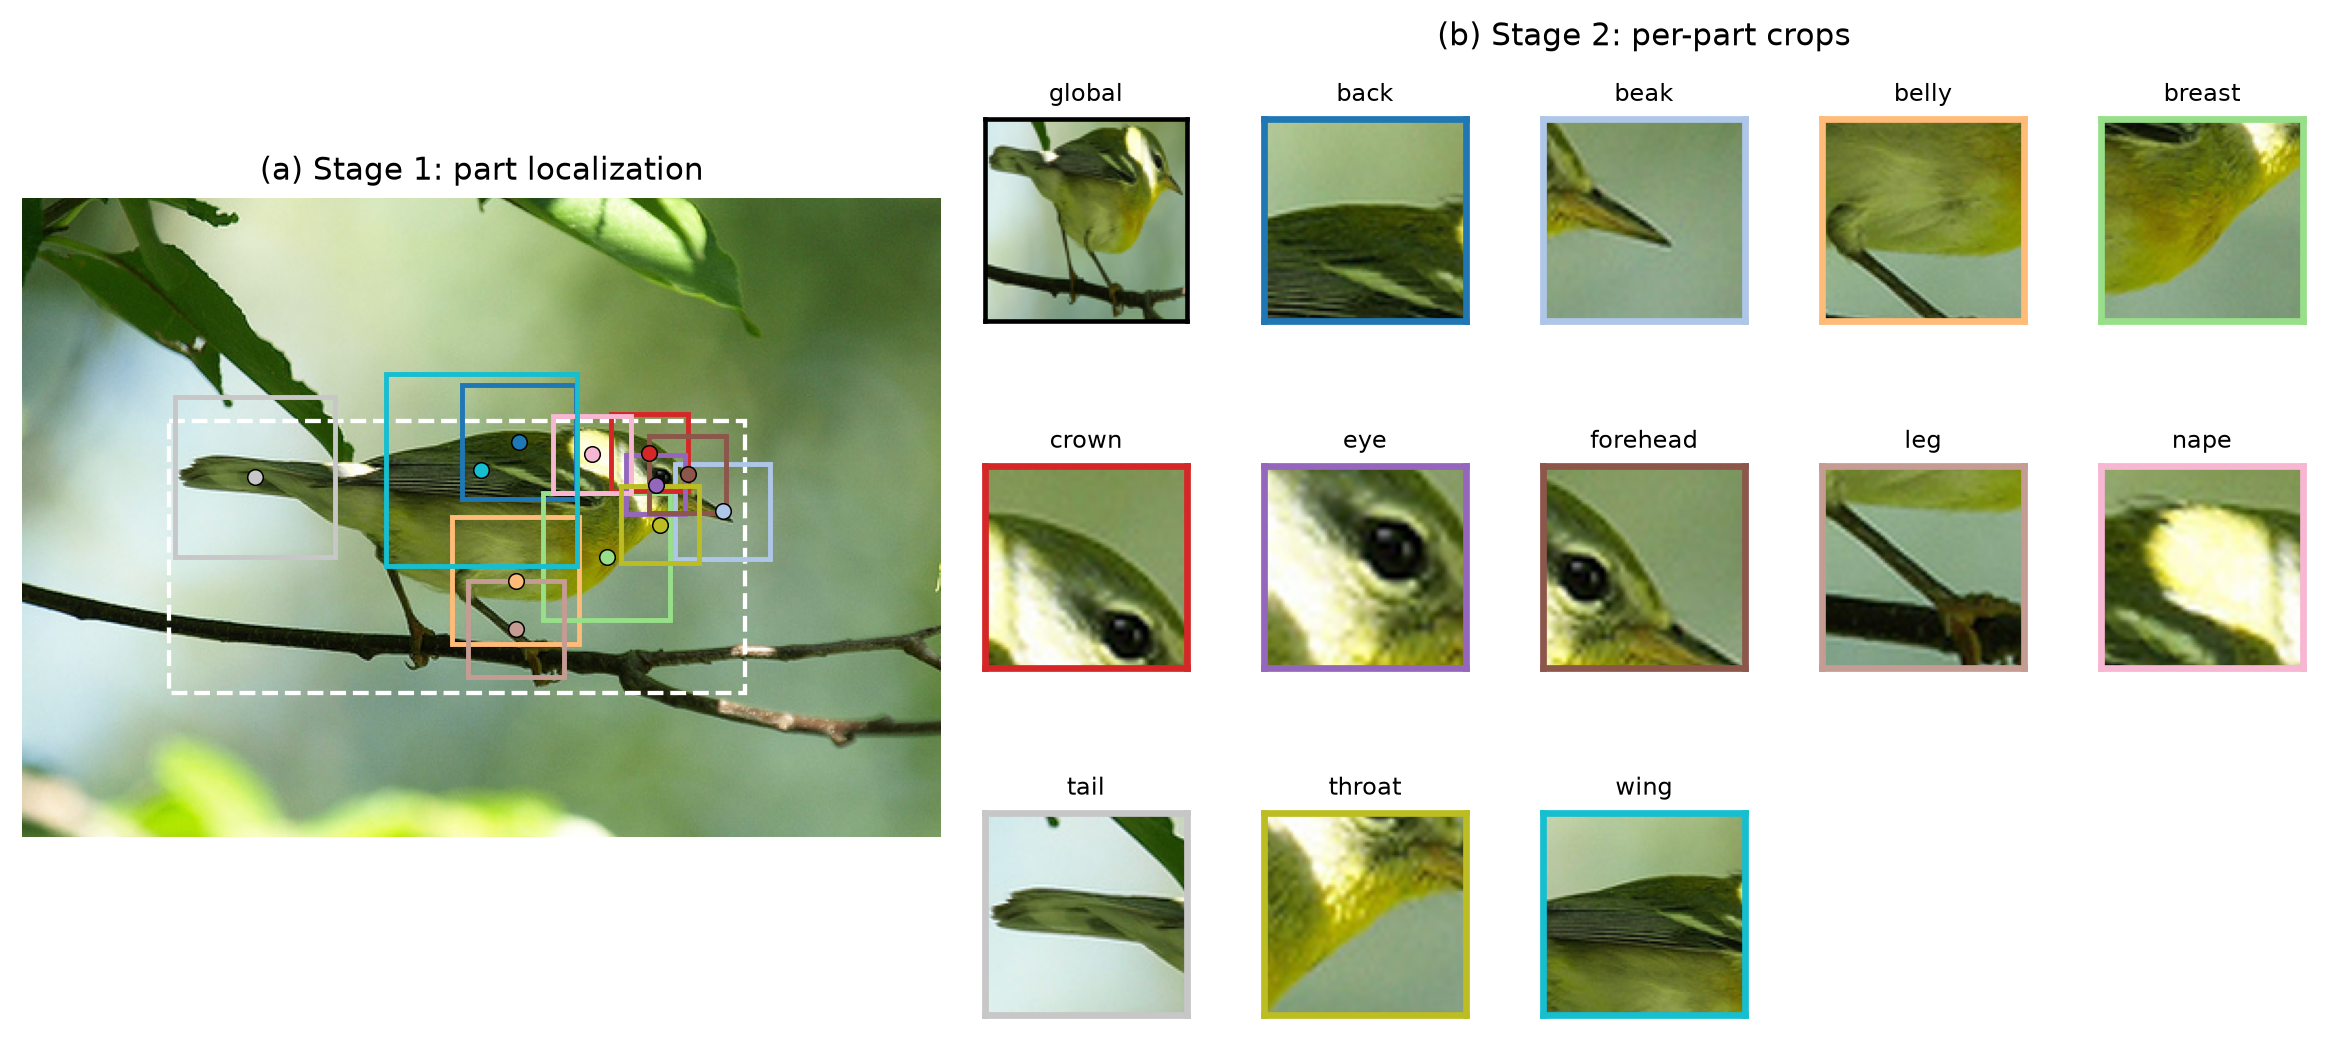
\includegraphics[width=0.62\textwidth]{part_crops}
  \caption{Part localisation (a) and the resulting per-part crops (b) on a
  CUB-200-2011 test image.}
  \label{fig:part-crops}
\end{figure*}

\textbf{Coarse-to-fine concepts.} On top of the grounded concepts we add
hierarchy \emph{within} the concept space for color and pattern attribute groups.
Instead of predicting the fine value directly, a small coarse head first
estimates a coarse colour family (e.g.\ warm / cool / neutral / iridescent);
its posterior is then concatenated with the part embedding and fed to a fine
head that predicts the specific value. This hierarchy acts on the concepts, not
on the species output.

\textbf{Training the classifier: independent vs.\ sequential.} The linear
species classifier is trained in two regimes that we compare throughout.
In the \emph{independent} regime it is fit on the ground-truth concept labels;
in the \emph{sequential} regime it is fit on the concept probabilities that the
concept encoder actually outputs, so that it can compensate for the encoder's
systematic errors. Both regimes are evaluated on the real concept predictions,
and the concept encoder itself is identical in both.

\textbf{Label-space hierarchy and mistake severity.} The 200 species form the
leaves of a taxonomic tree $\mathcal{T}$ obtained by mapping each class onto
WordNet (species\,$\rightarrow$\,genus\,$\rightarrow$\,family\,$\rightarrow
\cdots$)~\cite{miller1995wordnet}. For two nodes $a,b$ let $\mathrm{LCA}(a,b)$
denote their lowest common ancestor in $\mathcal{T}$, and let the \emph{height}
$h(v)$ of a node $v$ be the number of edges on the longest downward path from
$v$ to a leaf, so that $h(\cdot)=0$ for leaves. Following
\citet{bertinetto2020making}, the severity of predicting $\hat{y}$ when the true
class is $y$ equals the height of their LCA:
\begin{equation}
  s(y,\hat{y}) \;=\; h\!\left(\mathrm{LCA}(y,\hat{y})\right),
  \label{eq:cost}
\end{equation}
which is $0$ for a correct prediction, $1$ when the two species share a genus,
$2$ when they share only a family, and so on. The mistake severity we report is
the mean over all $N$ test examples:
\begin{equation}
  \mathrm{Sev} \;=\; \frac{1}{N}\sum_{i=1}^{N} s\!\left(y_i,\hat{y}_i\right)
  \;=\; \frac{1}{N}\sum_{i=1}^{N} h\!\left(\mathrm{LCA}(y_i,\hat{y}_i)\right),
  \label{eq:sev}
\end{equation}
so correct predictions contribute nothing and the score captures both how often
the model errs and how far its errors fall in the taxonomy (lower is better).

\textbf{Severity-aware decision (CRM).} The same cost drives the decision rule.
Let $p(c\mid x)$ be the model's softmax posterior over the $C{=}200$ classes.
Instead of the arg\,max, CRM~\cite{karthik2021nocost} returns the class of
minimum \emph{expected} severity:
\begin{equation}
  \hat{y}_{\mathrm{CRM}}
  \;=\; \arg\min_{k\in\{1,\dots,C\}} \sum_{c=1}^{C} s(k,c)\,p(c\mid x),
  \label{eq:crm}
\end{equation}
so that, when the model is uncertain, it favours a class that is taxonomically
close to the likely candidates rather than blindly picking the single most
probable one. Following \citet{karthik2021nocost}'s own formulation, we apply
CRM directly to an already-trained classifier's posterior: it is fully
post-hoc, adds no parameters, and requires no retraining.

\textbf{Metrics.} At the species level we report top-1 accuracy and the mistake
severity of Eq.~\eqref{eq:sev} (lower is better), which measures how
semantically close the errors are. At the concept level we report binary accuracy
and macro-averaged $F_1$ over the $109$ attributes for the concept encoder alone,
to check whether a numerically higher concept score reflects genuinely grounded
evidence or merely a class-correlated shortcut.

\section{Experiments and analysis}
\label{sec:experiments}
The experiments below separate two questions that a single accuracy number
conflates. First, does grounding the concept space in anatomy make the
bottleneck more faithful, and what does that faithfulness cost in raw
accuracy (Tables~\ref{tab:results} and~\ref{tab:concepts})? Second, once a
model exists, does structuring the label space change \emph{how} it is wrong,
independently of \emph{how often} (Table~\ref{tab:severity-breakdown})? The
two questions have different answers: concept-space structure trades accuracy
for faithfulness and, perhaps surprisingly, does not come with safer mistakes;
label-space structure buys safer mistakes almost for free.

\begin{table}[h]
  \centering
  \footnotesize
  \setlength{\tabcolsep}{4pt}
  \caption{Top-1 accuracy and mean WordNet mistake severity
  (Eq.~\eqref{eq:sev}, lower is better) on the CUB-200-2011 test set, under
  arg\,max and CRM.}
  \label{tab:results}
  \begin{tabular}{llcccc}
    \toprule
    & & \multicolumn{2}{c}{arg\,max} & \multicolumn{2}{c}{CRM} \\
    \cmidrule(lr){3-4}\cmidrule(lr){5-6}
    Variant & Classifier & Acc. & Sev. & Acc. & Sev. \\
    \midrule
    Black-box (reference) & --- & \textbf{85.83} & \textbf{0.326} & 85.66 & 0.330 \\
    \midrule
    \multirow{2}{*}{Flat}
      & Independent & 73.35 & 0.682 & 73.32 & 0.663 \\
      & Sequential  & 79.24 & 0.531 & 78.62 & 0.544 \\
    \addlinespace
    \multirow{2}{*}{Part-conditioned}
      & Independent & 73.14 & 0.795 & 73.21 & 0.777 \\
      & Sequential  & 73.68 & 0.763 & 73.68 & 0.741 \\
    \addlinespace
    \multirow{2}{*}{\;+ hierarchical concepts}
      & Independent & 72.26 & 0.822 & 72.04 & 0.814 \\
      & Sequential  & 72.23 & 0.803 & 69.02 & 0.937 \\
    \bottomrule
  \end{tabular}
  \par\vspace{2pt}
  {\scriptsize For reference on the severity scale, the WordNet cost matrix has a
  maximum of $7.0$ and a random classifier attains an expected severity of $5.59$.}
\end{table}

\textbf{The interpretability bottleneck has a measurable cost.} The black-box
outperforms every concept-based variant on \emph{both} accuracy and severity
(Table~\ref{tab:results}), and by a wide margin---if anything an
underestimate, since its checkpoint was early-stopped at epoch $18/30$ and had
not yet converged. This is the cost of interpretability already documented by
\citet{koh2020concept}: a $109$-dimensional concept vector is a real
information bottleneck, and forcing every prediction through it necessarily
throws away whatever visual shortcuts the unconstrained network would
otherwise use, however predictive they are. No concept-based variant closes
that gap, nor should we expect one to---the bottleneck is not a free
regularizer, it is a deliberate constraint traded for an inspectable
intermediate representation. The question the rest of this section asks is
what, exactly, that trade buys.

\begin{table*}[t]
  \centering
  \footnotesize
  \setlength{\tabcolsep}{4pt}
  \caption{Mistake-severity breakdown. Sev.\ (err.) is severity computed only
  over misclassified examples; Same-genus/Same-family/Far are the share of
  errors with LCA height $1$/$2$/$\geq 3$ \citep{bertinetto2020making}.}
  \label{tab:severity-breakdown}
  \begin{tabular}{llcccccccc}
    \toprule
    & & \multicolumn{4}{c}{arg\,max} & \multicolumn{4}{c}{CRM} \\
    \cmidrule(lr){3-6}\cmidrule(lr){7-10}
    Variant & Classifier & Sev.\ (err.) & Same-genus & Same-family & Far
                         & Sev.\ (err.) & Same-genus & Same-family & Far \\
    \midrule
    Black-box (reference) & --- & \textbf{2.303} & \textbf{29.4\%} & 10.8\% & \textbf{59.8\%}
                                 & 2.300 & 29.7\% & 11.0\% & 59.3\% \\
    \midrule
    \multirow{2}{*}{Flat}
      & Independent & 2.561 & 27.6\% & 9.7\%  & 62.7\% & 2.485 & 28.2\% & 9.6\%  & 62.2\% \\
      & Sequential  & 2.557 & 25.9\% & 11.5\% & 62.6\% & 2.545 & 26.1\% & 11.4\% & 62.5\% \\
    \addlinespace
    \multirow{2}{*}{Part-conditioned}
      & Independent & 2.960 & 23.1\% & 9.8\%  & 67.1\% & 2.900 & 23.3\% & 9.9\%  & 66.8\% \\
      & Sequential  & 2.900 & 23.0\% & 11.7\% & 65.3\% & 2.815 & 24.0\% & 11.8\% & 64.2\% \\
    \addlinespace
    \multirow{2}{*}{\;+ hierarchical concepts}
      & Independent & 2.965 & 22.7\% & 9.5\%  & 67.8\% & 2.912 & 22.9\% & 9.9\%  & 67.2\% \\
      & Sequential  & 2.891 & 23.2\% & 11.6\% & 65.2\% & 3.026 & 22.6\% & 11.0\% & 66.4\% \\
    \bottomrule
  \end{tabular}
\end{table*}

\textbf{Grounding costs on both fronts at once.} Table~\ref{tab:severity-breakdown}
splits Table~\ref{tab:results}'s severity into how often each model errs and,
conditioned on erring, how bad the mistake is. A natural hope would be that
grounding trades one for the other---errs more often, perhaps, but at least
fails gracefully onto a close relative when it does. That is not what happens.
Under arg\,max, the black-box's errors are not only the least frequent but
also, on average, the mildest and the most likely to stay within the true
genus; moving to part-conditioned and hierarchical concepts makes errors both
more frequent \emph{and} proportionally farther in the taxonomy (a larger Far
share, a smaller Same-genus share) than either the black-box or the flat
model. Grounding, in other words, does not fail more gracefully---it fails
more, and slightly worse per failure. A plausible reading is that the
whole-image context grounding removes is disproportionately useful for the
hardest calls: telling apart two closely related species often comes down to
subtle, correlated cues spread across the whole bird, which is exactly the
kind of evidence a part-local crop cannot see. Confirming that mechanism,
rather than just observing its signature, is a natural next step. CRM's effect
on this breakdown is uneven across variants, which we return to below.

\textbf{The sequential classifier usually outperforms the independent one.}
Training the species classifier on the concept encoder's own predictions
(sequential) rather than on the ground-truth labels (independent) raises top-1
accuracy and lowers severity for Flat and, more modestly, for
Part-conditioned; for $+$hierarchical concepts the two regimes are
statistically indistinguishable. The explanation is straightforward: the
sequential classifier is trained on the same noisy concept probabilities it
will see at test time, so it can absorb the concept encoder's systematic
biases, whereas the independent classifier, fit on clean labels, faces a
train--test mismatch it never learns to correct. Adding the coarse-to-fine
gate evidently leaves little of that mismatch for the sequential classifier to
absorb, which is why the gap closes there. Because the sequential regime gives
each variant its best or tied-best performance, we read the effect of
grounding from that column.

\textbf{Grounding concepts reduces accuracy---by design.} Within the
sequential regime, accuracy falls step by step as we add structure: flat,
then part-conditioned, then $+$hierarchical, with severity rising in tandem.
This is expected rather than a shortcoming. The flat model's edge comes partly
from whole-image, class-correlated shortcuts that part conditioning
deliberately removes---the same shortcuts Table~\ref{tab:concepts} will show
inflating its apparent concept quality. The concept-space design trades a few
accuracy points for a bottleneck that is actually faithful: each concept is
grounded in the body region it names and cannot circularly infer the answer
from global cues, and colour/pattern concepts are additionally organised
hierarchically---an interpretability benefit no accuracy number captures.

\begin{table}[h]
  \centering
  \footnotesize
  \caption{Concept-level accuracy and macro-$F_1$ over the $109$ attributes,
  for each concept encoder alone.}
  \label{tab:concepts}
  \begin{tabular}{lccc}
    \toprule
    Concept encoder & \# concepts & Acc.\ (\%) & Macro-$F_1$ \\
    \midrule
    Flat                          & 109 & \textbf{95.66} & \textbf{0.876} \\
    Part-conditioned              & 109 & 91.36 & 0.758 \\
    \; + hierarchical concepts    & 109 & 91.24 & 0.753 \\
    \bottomrule
  \end{tabular}
\end{table}

\textbf{Higher concept scores do not imply more faithful concepts.}
Table~\ref{tab:concepts} evaluates concept quality in isolation, and the flat
encoder comes out well ahead of the part-conditioned one---even though the
latter is the one that actually breaks prediction circularity. Far from
contradicting our thesis, this gap \emph{supports} it: the flat encoder can
infer an attribute from whole-image cues that are diagnostic of the species
(e.g.\ recognising \emph{wing color} from the overall plumage pattern) rather
than from the region the attribute names, the same shortcut mechanism that
inflates its species accuracy in Table~\ref{tab:results}. The part-conditioned
encoder, forced to work from the crop of the relevant body part alone, cannot
take that shortcut; its lower score is therefore a more honest measurement of
whether the concept is grounded in its own evidence, not a worse one. A
high concept score, on its own, is consequently not evidence of a faithful
bottleneck---it can equally be evidence of leakage. Adding the coarse-to-fine
gate barely moves the number either way: the extra structure is essentially
free.

\textbf{CRM buys lower severity almost everywhere, for almost no accuracy.}
Applied exactly as \citet{karthik2021nocost} define it---no retraining,
no extra parameters, no free choices---CRM lowers severity for five of the six
concept-based rows in Table~\ref{tab:results}, in every case at a cost of well
under half an accuracy point. It leaves the black-box and Flat-Sequential
essentially unchanged: both already have sharp, confident posteriors, so there
is little uncertainty left for a severity-aware re-ranking to act on.
$+$Hierarchical-Sequential is the one row where CRM makes both accuracy and
severity worse. A re-ranking rule built from expected severity is only as
good as the posterior it re-ranks; when that posterior is not a faithful
estimate of the model's own uncertainty, minimising \emph{expected} severity
under it can easily miss actual severity. CRM's benefit is therefore real but
conditional on the classifier it is layered onto, not a property of the
decision rule alone---exactly the caveat a severity-aware method should be
reported with.

\section{Conclusions}
We introduced hierarchical structure into a supervised CBM along two
axes---part-grounded, coarse-to-fine concepts in the concept space, and a
WordNet taxonomy with an LCA severity metric plus a post-hoc CRM decision rule
in the label space. Compared with an unconstrained black-box, the concept
bottleneck costs both accuracy and severity, the well-documented price of
interpretability.

The two concept-space changes do not pay off equally. Adding the
coarse-to-fine concept hierarchy on top of part conditioning underperforms
our expectations: it does not improve accuracy or severity over plain part
conditioning (Table~\ref{tab:results}), and on the concept consistency test
it is no better, and slightly worse, at landing on the exact edited colour
(Table~\ref{tab:crown-intervention}). Part conditioning alone is the more
promising direction: at a modest accuracy cost, it makes concepts far more
consistent with the local evidence they name.

CRM lowers mistake severity at test time at virtually no accuracy cost on
most variants, provided the classifier it is layered onto gives it a
reasonably faithful posterior. Future work: hierarchy-aware training losses,
real part segmentation in place of keypoint-centred crops, a broader concept
consistency test covering more attributes and edits, and pairing CRM with a
hierarchically structured classifier head.


%%
%% The next two lines define the bibliography style to be used, and
%% the bibliography file.
\bibliographystyle{ACM-Reference-Format}
\bibliography{bib/biblio}

\end{document}
